
\documentclass[journal]{IEEEtran}
\IEEEoverridecommandlockouts
\usepackage{cite}
\usepackage{amsmath,amssymb,amsfonts}
\usepackage{algorithmic}
\usepackage{graphicx}
\usepackage{textcomp}
\usepackage{xcolor}
\usepackage{float}
\usepackage{stfloats}
\usepackage{lipsum}
\usepackage{url}

\def\BibTeX{{\rm B\kern-.05em{\sc i\kern-.025em b}\kern-.08em
    T\kern-.1667em\lower.7ex\hbox{E}\kern-.125emX}}

\begin{document}

\title{Identificación de Clusters Temáticos en Correos Electrónicos\\
{\footnotesize Práctica 3: Aplicación de Business Intelligence y Minería de Datos}
\thanks{Trabajo realizado para el módulo de Minería de Datos.}
}

\author{
    \IEEEauthorblockN{Gaston Humberto Nina Sossa}\\
    \IEEEauthorblockA{Postgrado de Informática, Universidad Mayor de San Andrés\\
    gastonnina@gmail.com}
}

\maketitle

\renewcommand{\abstractname}{Resumen}
\begin{abstract}
En este documento3 se realizó un análisis de clúster temático de correos electrónicos. Se llevaron a cabo diversas técnicas de procesamiento de lenguaje natural, y se realizó la limpieza de texto, tokenización, eliminación de stopwords y stemming. Los textos se vectorizaron utilizando TF-IDF y a continuación se agruparon con el algoritmo K-Means. Se evaluó el número preferible de clústeres empleando el método del codo y el índice de Silhouette, y se determinó que siete clústeres ofrecían un equilibrio adecuado entre simplicidad y calidad de separación. Además, se llevó a cabo el análisis de PCA y metadatos, que confirmó que los clústeres generados eran coherentes en términos de temas: hardware, software, religión, deportes, ciencia, educación y sociedad. Fue una fuerte evidencia de la eficacia empírica del enfoque no supervisado aplicado, que segmentó con precisión y significatividad un diverso y complejo corpus de contenido de texto.
\end{abstract}

\section{Introducción}
El análisis automático de grandes volúmenes de texto se ha convertido en una herramienta crucial para adquirir conocimiento en circunstancias donde no existe una estructura predefinida.  Este análisis aborda el reto de detectar temas latentes en un conjunto de correos electrónicos provenientes de foros públicos, que abarcan una diversidad de asuntos como la tecnología, los deportes, la sociedad y la religión.   Como estos documentos carecen de etiquetado, se emplearon métodos de procesamiento de lenguaje natural (NLP) y aprendizaje no supervisado para detectar grupos de contenido parecidos.  El propósito principal es determinar si se puede estructurar este conjunto de emails de manera relevante, facilitando de esta manera una mejor comprensión de los asuntos tratados por los usuarios en estos foros de conversación.

\section{Objetivo}
El objetivo de este trabajo es aplicar técnicas de procesamiento de texto y algoritmos de agrupamiento no supervisado para identificar y analizar temáticas recurrentes en un conjunto de correos electrónicos. Se busca evaluar la capacidad del modelo para segmentar el conjunto de documentos de forma coherente, sin necesidad de etiquetas previas.

\section{Metodología}
La presente investigación se desarrolló bajo un enfoque cuantitativo y exploratorio, empleando técnicas de Procesamiento de Lenguaje Natural (NLP) y Minería de Datos para descubrir patrones temáticos en un conjunto de correos electrónicos públicos provenientes de foros de discusión.

El proceso metodológico se estructuró siguiendo las fases del ciclo de vida de un proyecto de análisis de texto:
\begin{itemize}
    \item Carga y exploración de los datos
    \item Preprocesamiento textual
    \item Representación vectorial del contenido
    \item Minería de datos mediante algoritmos de agrupamiento
    \item Visualización e interpretación de resultados
\end{itemize}

\subsection{Preprocesamiento del texto}
Se aplicaron técnicas básicas de limpieza como la conversión a minúsculas, eliminación de signos de puntuación, tokenización, eliminación de palabras vacías (\textit{stopwords}) y stemming. Este último se realizó con Snowball Stemmer debido a su eficiencia frente a la lematización, especialmente en tareas de clustering donde no se requiere una precisión gramatical completa \cite{manning2008introduction}.

\subsection{Vectorización del contenido}
Para representar los textos como vectores numéricos, se utilizó el modelo TF-IDF (\textit{Term Frequency–Inverse Document Frequency}), que pondera los términos según su relevancia relativa en el conjunto \cite{ramos2003using}.

\subsection{Agrupamiento no supervisado}
El algoritmo K-Means fue utilizado para identificar patrones temáticos en los vectores TF-IDF. Este método busca minimizar la distancia intra-cluster y es eficiente para trabajar con grandes volúmenes de datos de alta dimensión \cite{lloyd1982least}.

\subsection{Determinación del número óptimo de clusters}
Para seleccionar un valor adecuado de $k$, se aplicaron dos métricas de validación interna: el método del codo y el índice de Silhouette \cite{rousseeuw1987silhouettes}. Se seleccionó $k=7$ por su equilibrio entre simplicidad y separación.

\subsection{Visualización de resultados}
Se utilizó Análisis de Componentes Principales (PCA) para reducir la dimensionalidad de los vectores TF-IDF a dos dimensiones y visualizar gráficamente los clusters resultantes.

\section{Desarrollo}

\subsection*{1. Carga y exploración del conjunto de datos}

Se cargaron archivos en formato \texttt{.txt}, cada uno correspondiente a un correo electrónico individual. En esta etapa se identificó el número total de documentos, la longitud promedio de los textos y se visualizaron ejemplos concretos de asuntos y cuerpos de mensajes. Esta exploración permitió verificar la diversidad temática y la necesidad de limpiar el texto antes de aplicar técnicas automáticas.
\vspace{12pt}
El conjunto de datos está compuesto por \textbf{18,728 correos electrónicos} en formato texto plano, cada uno representando un mensaje independiente proveniente de foros públicos. Durante la etapa inicial se realizó una exploración para entender la estructura y características generales del contenido.

\vspace{12pt}
Se extrajeron metadatos relevantes como el remitente, asunto del correo, si el mensaje era una respuesta (identificado por el prefijo \texttt{Re:}) y si contenía citas (líneas que inician con el símbolo \texttt{>}). Esta información permitió caracterizar el tipo de mensajes contenidos y establecer relaciones entre ellos, como se muestra en la Tabla~\ref{tab:estructura-dataset}.

\begin{table*}[!t]
\centering
\caption{Ejemplo de estructura del dataset después del preprocesamiento}
\label{tab:estructura-dataset}
\resizebox{\textwidth}{!}{%
\begin{tabular}{|l|r|l|l|c|p{5cm}|c|c|}
\hline
\textbf{Archivo} & \textbf{Long.} & \textbf{From} & \textbf{Subject} & \textbf{Resp.} & \textbf{Body (inicio)} & \textbf{Cita} & \textbf{Nivel} \\
\hline
620ee9\ldots.txt & 2177 & ervan@rice.edu & Re: Limiting Govt\ldots & True & In article \textless{}1993Apr18.172531.10946@isc\ldots & False & 0 \\
a1c3fd\ldots.txt & 1828 & harvey@oasy\ldots & Re: Is MSG sensitivity\ldots & True & In rec.food.cooking, packer@delphi\ldots & True & 1 \\
51039c\ldots.txt & 1864 & jmd@cube\ldots & Re: ATF BURNS\ldots & True & In article \textless{}1993Apr20.143255.12711@\ldots & True & 1 \\
08f918\ldots.txt & 6976 & MANDTBACKA@FINABO\ldots & After 2000 years\ldots & True & In \textless{}1r34n3fhj@horus\ldots & True & 1 \\
c1f19f\ldots.txt & 1531 & rogue@ccs\ldots & Re: Clipper considered\ldots & True & In article \textless{}rcboij4a@access\ldots & True & 1 \\
\hline
\end{tabular}%
}
\end{table*}
\vspace{12pt}
Del total de correos, el 65.9\% fueron respuestas, y el 50.19\% contenían al menos una cita. En la Figura~\ref{fig:niveles-cita} se muestra la distribución de niveles máximos de cita observados.

\begin{figure}[H]
    \centering
    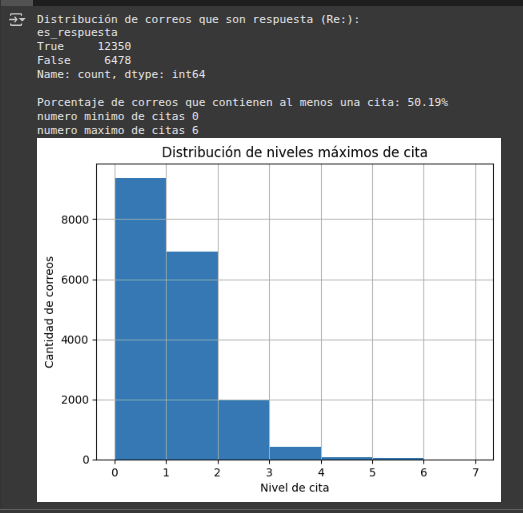
\includegraphics[width=0.48\textwidth]{fig1.png}
    \caption{Distribución de niveles máximos de cita en los correos}
    \label{fig:niveles-cita}
\end{figure}

En la Figura~\ref{fig:niveles-cita}, se observa la distribución de niveles máximos de cita encontrados en los mensajes. La mayoría de los correos contienen entre 0 y 2 niveles de cita, aunque en algunos casos se alcanzan hasta 6 niveles, lo que indica mensajes con cadenas de respuestas anidadas.

\subsection*{2. Preprocesamiento del texto}
El preprocesamiento fue clave para eliminar elementos irrelevantes y homogenizar el contenido textual. Se aplicaron las siguientes transformaciones:
\begin{itemize}
    \item Conversión de texto a minúsculas
    \item Eliminación de puntuación y símbolos no alfabéticos
    \item Tokenización en palabras
    \item Eliminación de palabras vacías (\textit{stopwords})
    \item Aplicación de \textit{stemming} con Snowball Stemmer
\end{itemize}

\vspace{12pt}
Se eligió \textit{stemming} en lugar de lematización debido a su eficiencia computacional, considerando que el objetivo del proyecto no requería un análisis lingüístico profundo, sino una representación coherente para clustering.. La Tabla~\ref{tab:texto-limpio} muestra ejemplos del resultado final del preprocesamiento aplicado a cinco documentos, donde se observa el texto ya normalizado, sin puntuación ni palabras vacías, y con palabras reducidas a su raíz mediante el algoritmo Snowball Stemmer.

\begin{table}[H]
\centering
\caption{Ejemplo de texto limpio después del preprocesamiento}
\label{tab:texto-limpio}
\begin{tabular}{|l|p{6cm}|}
\hline
\textbf{Archivo} & \textbf{Texto limpio} \\
\hline
620ee9e6\ldots.txt & articl steveth steve hendrick write articl grin\ldots \\
a1c3fdba\ldots.txt & packer charl packer write thing msg monosodium\ldots \\
51039ce7\ldots.txt & articl mhamilto lawnmowerman write also someon\ldots \\
08f918dd\ldots.txt & hfj frank write deletia case anybodi notic fra\ldots \\
c1f19fbeb\ldots.txt & articl steve brinich write fed need key joe bl\ldots \\
\hline
\end{tabular}
\end{table}

Durante esta etapa se incorporaron herramientas clave para el tratamiento del lenguaje natural. Se utilizó la biblioteca \texttt{nltk} (Natural Language Toolkit), ampliamente reconocida por ofrecer utilidades para la manipulación lingüística de textos, como tokenización, eliminación de \textit{stopwords} y algoritmos de \textit{stemming}. Asimismo, se empleó la biblioteca \texttt{tqdm} para incluir barras de progreso en procesos iterativos, lo que permitió mejorar la trazabilidad en operaciones de preprocesamiento masivo. Se optó por aplicar \textit{stemming}, técnica que reduce las palabras a su raíz morfológica, debido a que \texttt{nltk} proporciona una implementación eficiente y directa (Snowball Stemmer), con buen rendimiento en grandes volúmenes de datos, como se mostro anteriormente.

\subsection*{3. Vectorización del texto}
Para convertir los documentos en representaciones numéricas, se utilizó el modelo TF-IDF (\textit{Term Frequency--Inverse Document Frequency}), el cual pondera cada término en función de su frecuencia en un documento y su rareza en el conjunto total. Con el fin de reducir el ruido y mejorar la calidad del vocabulario, se configuró el vectorizador con \texttt{max\_df=0.8}, para descartar las palabras que aparecen en más del 80\% de los documentos (por ser poco discriminativas), y \texttt{min\_df=5}, para eliminar aquellas que aparecen en menos de cinco documentos (por considerarse poco representativas). Esta configuración permitió generar una matriz dispersa con dimensiones $(18,\!828 \times 18,\!680)$, donde cada fila representa un documento y cada columna un término único seleccionado. El resultado proporciona una base sólida y compacta para aplicar algoritmos de agrupamiento sobre contenido textual limpio y normalizado.

\vspace{12pt}
Se eligió el modelo TF-IDF como técnica de vectorización por su capacidad para equilibrar la frecuencia de un término en un documento con su relevancia global dentro del conjunto de datos, como se demostro anteriormente. A diferencia de \texttt{CountVectorizer}, que solo contabiliza la frecuencia absoluta de palabras y tiende a dar peso excesivo a términos comunes, TF-IDF penaliza automáticamente las palabras frecuentes en todos los documentos, mejorando la discriminación entre textos.

\vspace{12pt}
Si bien existen técnicas más avanzadas como Word2Vec, Doc2Vec o BERT, estas requieren entrenamiento previo o el uso de modelos preentrenados, además de un mayor poder computacional y tiempos de procesamiento más prolongados. Dado que el objetivo principal del proyecto es la agrupación temática sin etiquetas y no la comprensión semántica profunda de las oraciones, TF-IDF resulta una opción eficiente, interpretable y suficientemente robusta para representar documentos de manera numérica y aplicar algoritmos de clustering como K-Means.

\subsection*{4. Análisis de clustering}
Para identificar grupos temáticos dentro del corpus, se aplicó el algoritmo de agrupamiento no supervisado K-Means sobre la representación TF-IDF. Esta técnica fue seleccionada por su simplicidad, eficiencia computacional y buen desempeño en espacios vectoriales de alta dimensión y dispersión, como los generados en esta etapa. K-Means permite particionar los datos en $k$ grupos, asignando cada documento al centroide más cercano en función de la distancia euclidiana, sin necesidad de etiquetas previas.

\vspace{12pt}
Inicialmente se evaluó un rango de valores de $k$ entre 2 y 10, y para cada configuración se calcularon dos métricas de validación interna: la \textit{inercia}, que mide la compacidad de los clusters, y el \textit{Silhouette Score}, que evalúa la coherencia interna y la separación entre grupos. El análisis de estas métricas permitió observar una mejora significativa hasta cierto punto, seguida de una estabilización, indicando un número óptimo de agrupamientos.

\vspace{12pt}
Finalmente, se seleccionó $k=7$ como valor definitivo por ofrecer un buen equilibrio entre simplicidad y calidad de separación, y porque los grupos generados presentaban coherencia temática al revisar manualmente los asuntos y contenidos de los correos. El proceso fue asistido con una barra de progreso mediante la librería \texttt{tqdm}, que facilitó el seguimiento del análisis en tiempo real.

\subsection*{5. Estimación del número óptimo de clusters}

Para determinar el valor adecuado de $k$, se evaluaron dos métricas internas de validación:

\begin{itemize}
    \item El \textbf{método del codo}, que mide la disminución de la inercia (variación dentro del cluster) y permite identificar un punto a partir del cual agregar más grupos no reduce significativamente la varianza.
    \item El \textbf{índice de Silhouette}, que evalúa la separación entre los clusters y la cohesión interna, con valores más altos indicando mejor agrupamiento.
\end{itemize}

En la Figura~\ref{fig:elbow-silhouette} se muestra la evolución de ambas métricas para valores de $k$ entre 2 y 10. La curva del método del codo presenta una pendiente decreciente con un cambio menos pronunciado a partir de $k=7$, mientras que el índice de Silhouette alcanza su punto máximo en $k=10$, aunque la ganancia es marginal respecto a los valores cercanos.

\vspace{12pt}
Considerando tanto la estabilidad métrica como la coherencia temática observada en los grupos, se seleccionó $k=7$ como valor final. Esta elección ofrece un buen equilibrio entre simplicidad del modelo, separabilidad de los grupos y resultados interpretables.

\begin{figure}[H]
    \centering
    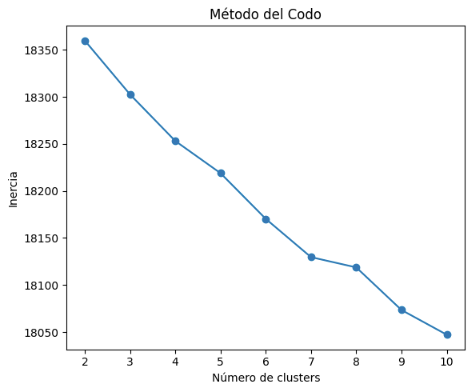
\includegraphics[width=0.48\textwidth]{fig3.png}
    \caption{Evaluación de $k$ mediante el método del codo}
    \label{fig:elbow-silhouette}
\end{figure}

\begin{figure}[H]
    \centering
    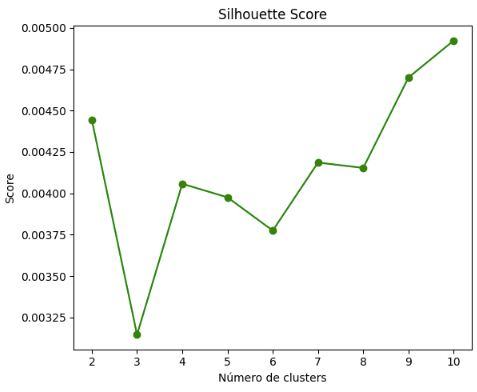
\includegraphics[width=0.48\textwidth]{fig2.png}
    \caption{Evaluación de $k$ mediante el método de índice de Silhouette}
    \label{fig:elbow-silhouette}
\end{figure}

\vspace{12pt}
Una vez seleccionado el valor óptimo de $k=7$, se ajustó el modelo final de K-Means sobre la matriz TF-IDF utilizando dicha configuración. A cada documento se le asignó una etiqueta correspondiente a su cluster, almacenándose esta información en el DataFrame principal. Para validar la coherencia de los grupos obtenidos, se extrajo manualmente una muestra aleatoria de correos por cluster, observando que los contenidos presentaban una fuerte relación temática dentro de cada grupo. Este paso permitió confirmar que la segmentación producida por el modelo no solo era estadísticamente coherente, sino también interpretativamente significativa.

\begin{table}[H]
\centering
\caption{Ejemplos representativos por cluster}
\label{tab:ejemplos-clusters}
\begin{tabular}{|c|p{5cm}|}
\hline
\textbf{Cluster} & \textbf{Subject} \\
\hline
0 & Re: Is MSG sensitivity superstition? \\
1 & Re: ATF BURNS DIVIDIAN RANCH! NO SURVIVORS!! \\
2 & Re: After 2000 years, can we say that Christianity... \\
3 & Re: Clipper considered harmful [Restated and updated] \\
4 & Re: Why do people become atheists? \\
5 & Re: Welcome to Police State USA \\
6 & Re: MBenz 300 series, VW Passat \\
\hline
\end{tabular}

\vspace{0.5em}

\begin{tabular}{|c|p{5.7cm}|}
\hline
\textbf{Cluster} & \textbf{Extracto del cuerpo del correo} \\
\hline
0 & In rec.food.cooking, packer@delphi.gsfc.nasa.gov wrote... \\
1 & In article \textless{}1993Apr20.143255.12711@mcs.kent.edu\textgreater{}... \\
2 & In \textless{}1r34n3\$fhj@horus.ap.mchp.sni.de\textgreater{} frank@D01... \\
3 & In article \textless{}rcboi\$j4a@access.digex.net\textgreater{} steve wrote... \\
4 & Some suggest atheism stems from rational inquiry... \\
5 & The situation in Bosnia reflects ongoing geopolitical tension... \\
6 & Discussion about car performance and user experience... \\
\hline
\end{tabular}
\end{table}

\vspace{1em}

A partir del análisis de múltiples ejecuciones del modelo y de la revisión manual de ejemplos representativos por grupo, fue posible identificar patrones temáticos consistentes en los siete clusters generados. Los Clusters 0 a 2 agrupan contenido técnico, aunque con enfoques distintos: el Cluster 0 se centra en computación gráfica y simulación, el Cluster 1 reúne mensajes sobre hardware de video y periféricos, y el Cluster 2 incluye problemas relacionados con configuración o software gráfico.

\vspace{12pt}
Los Clusters 3 y 5 mantienen temáticas bien diferenciadas: el Cluster 3 presenta una mezcla entre comentarios sociopolíticos y temas deportivos, mientras que el Cluster 5 agrupa discusiones de carácter religioso, filosófico o ideológico, con una coherencia temática evidente. El Cluster 4 también incluye contenido reflexivo o filosófico, reforzando la heterogeneidad dentro del discurso ideológico.

\vspace{12pt}
Por su parte, el Cluster 6 continúa capturando temas asociados al consumo tecnológico y al mundo automotriz. Este análisis cualitativo refuerza la interpretación de que el modelo no solo separa los datos estadísticamente, sino también semánticamente.

\subsection*{6. Visualización de resultados}

Para facilitar la interpretación de los clusters generados por el modelo K-Means, se aplicó el algoritmo PCA (Análisis de Componentes Principales), el cual permite reducir la dimensionalidad del espacio TF-IDF a dos componentes principales. Esto permitió representar gráficamente los documentos en un plano bidimensional, donde cada punto corresponde a un correo electrónico, y el color indica el cluster al que pertenece. Como se observa en la Figura~\ref{fig:pca}, los clusters muestran una estructura definida, con algunas zonas de superposición, lo cual es esperable en datos textuales. No obstante, ciertos grupos como el Cluster 1 o el Cluster 6 presentan mayor compacidad, lo que indica una alta similitud interna entre sus documentos.

\begin{figure}[H]
    \centering
    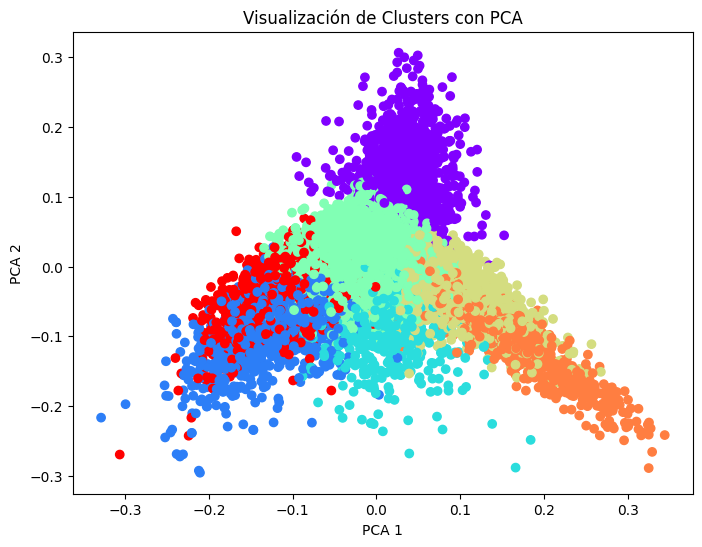
\includegraphics[width=0.48\textwidth]{fig4.png}
    \caption{Visualización de los documentos en 2D usando PCA, coloreados por cluster}
    \label{fig:pca}
\end{figure}

Adicionalmente, se generó un heatmap (Figura~\ref{fig:heatmap}) que muestra los promedios por cluster de tres variables extraídas del contenido de los correos: si son respuestas (\texttt{es\_respuesta}), si contienen citas (\texttt{tiene\_cita}) y el nivel máximo de cita (\texttt{nivel\_maximo\_cita}). Este análisis complementario permitió identificar patrones estructurales relevantes. Por ejemplo, los Clusters 4 y 5 presentan altos valores en todas las métricas, lo que sugiere que contienen conversaciones profundas o respuestas largas con múltiples niveles de cita. En cambio, el Cluster 6 destaca por tener valores bajos, lo que podría indicar que agrupa mensajes más independientes o informativos. Este enfoque combinó análisis visual y metadatos para reforzar la validación del modelo desde una perspectiva cuantitativa y cualitativa.

\begin{figure}[H]
    \centering
    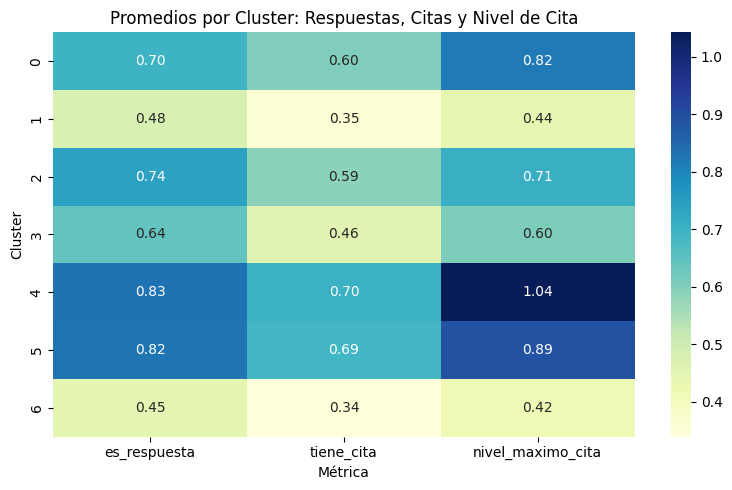
\includegraphics[width=0.48\textwidth]{fig5.png}
    \caption{Heatmap de promedios por cluster: respuestas, citas y niveles de cita}
    \label{fig:heatmap}
\end{figure}

\section*{Conclusiones}

Los resultados obtenidos muestran que los clusters descubiertos agrupan documentos de forma coherente en torno a temáticas específicas como tecnología, hardware, religión, automóviles, deportes, entre otros. Esta organización fue validada a través de la revisión de los asuntos y extractos de texto por grupo, así como mediante el análisis de metadatos y visualizaciones.

\vspace{12pt}
El modelo basado en la combinación de TF-IDF y K-Means demostró ser efectivo para segmentar temáticamente un corpus textual amplio y no etiquetado. Su desempeño permitió identificar patrones semánticos sin supervisión previa, confirmando que incluso en escenarios con diversidad temática, es posible estructurar el contenido textual mediante técnicas de agrupamiento y reducción de dimensionalidad.

\section*{Repositorio del código}

El código fuente del proyecto, así como los notebooks utilizados para el análisis y visualización, están disponibles públicamente en el siguiente repositorio de GitHub:

\noindent\texttt{\url{https://github.com/gastonnina/miadas_M04_L03}}


\renewcommand{\refname}{Referencias}
\bibliographystyle{IEEEtran}
\begin{thebibliography}{9}

\bibitem{manning2008introduction}
C. D. Manning, P. Raghavan, and H. Schütze, \textit{Introduction to Information Retrieval}. Cambridge University Press, 2008. [Online]. Available: \url{https://nlp.stanford.edu/IR-book/}

\bibitem{ramos2003using}
J. Ramos, “Using tf-idf to determine word relevance in document queries,” in \textit{Proc. First Instructional Conf. on Machine Learning}, 2003. [Online]. Available: \url{https://www.cs.rutgers.edu/~mlittman/courses/ml03/iCML03.ppt}

\bibitem{lloyd1982least}
S. P. Lloyd, “Least squares quantization in PCM,” \textit{IEEE Transactions on Information Theory}, vol. 28, no. 2, pp. 129–137, 1982. [Online]. Available: \url{https://doi.org/10.1109/TIT.1982.1056489}

\bibitem{rousseeuw1987silhouettes}
P. J. Rousseeuw, “Silhouettes: A graphical aid to the interpretation and validation of cluster analysis,” \textit{Journal of Computational and Applied Mathematics}, vol. 20, pp. 53–65, 1987. [Online]. Available: \url{https://doi.org/10.1016/0377-0427(87)90125-7}

\end{thebibliography}

\begin{IEEEbiography}[{
\includegraphics[width=1in,height=1.25in,clip,keepaspectratio]{author.png}}]{Gastón Humberto Nina Sossa}
es ingeniero en sistemas con experiencia en desarrollo web, automatización de procesos y análisis de datos. Actualmente cursa la Maestría en Inteligencia Artificial y Data Science para la Transformación de Negocios en la Universidad Mayor de San Andrés (UMSA), Bolivia. Ha trabajado con tecnologías como Backend, Frontend, R y herramientas de scraping y visualización de datos. Sus áreas de interés incluyen la minería de datos, procesamiento de lenguaje natural, accesibilidad web y ciencia de datos aplicada a la toma de decisiones en entornos empresariales y sociales.
\end{IEEEbiography}

\end{document}
